\documentclass[a6paper, 10pt, twoside]{article}
%\usepackage[T1]{fontenc}
\usepackage[british]{babel}
\usepackage[utf8]{inputenc}
\usepackage{float, graphicx,amsmath,amsfonts,cite,enumerate,tabularx}
\usepackage[final]{pdfpages}
\usepackage{wrapfig}
\usepackage[margin=0.3in]{geometry}
\usepackage{sidspaltHack}
\usepackage{digital}

\setlength{\oddsidemargin}{-0.37in}
\setlength{\evensidemargin}{-0.47in}
\setlength{\textwidth}{215pt}

\pagestyle{empty}

\begin{document}
\nysida{5}{1}
\noindent
\chaptertitlenobr{E$\varepsilon$}{Visor till vin}
\small
\begin{center}
\songtitle{$\varepsilon1$}{Vinets lov} 
\mel{Fjäriln vingad}
\end{center}
\begin{lyrics}
När det strålar uti salen\\
utav glädje glans och färg.\\
När det gnistrar uti pokalen\\
utav ädla druvors märg.
\vspace{5pt}\\
Kära vänner varför dröja\\
med att dricka glädjen till.\\
Låt oss bortom framtids slöja\\
se allt skönt vi skåda vill.
\vspace{5pt}\\
Drick för allt som livet skänker,\\
glädjestunder, ljus och sol.\\
Drick för stjärnorna som blänker\\
över oss från pol till pol.
\vspace{5pt}\\
Drick för våren, väl du kan det.\\
Drick för värmen våren ger.\\
Drick för starka vänskapsbanden.\\
Drick för allt vad skönt du ser.
\end{lyrics}

\nysida{5}{2}
\noindent
\begin{center}
\songtitle{$\varepsilon2$}{Feta fransyskor} 
\mel{Marche Militaire (Tomatarnas vaktparad)}
\end{center}
\begin{lyrics}
Feta fransyskor \\
som svettas om fötterna\\
de trampar druvor \\
som sedan skall jäsas till vin!\\
Transpirationen viktig e', \\
ty den ger fin bouquet.\\
Vårtor och svampar följer med, \\
men vad gör väl det?\\
För \\
vi vill ha vin, vill ha vin, \\
vill ha mera vin,\\
även om följderna bli\\
att vi må lida pin!
\vspace{5pt}\\
\textit{Damer:} Flaskan och glasen har gått i sin!\\
\textit{Herrar:} Hit med vin, mera vin!\\
\textit{Damer:} Tror ni att vi är fyllesvin?\\
\textit{Herrar:} JA, fast större! 
\end{lyrics}
\begin{flushright}
K-LTH, Sångarstriden 1985
\end{flushright}
\vfill
\begin{figure}[!h]
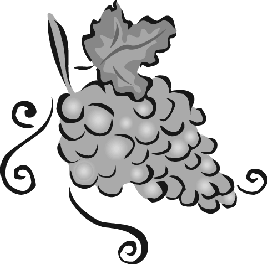
\includegraphics[width=0.5\textwidth]{grapes.png}
\end{figure}

\nysida{5}{3}
\noindent
\begin{center}
\songtitle{$\varepsilon3$}{Vinvisa} 
\mel{Amanda Lundbom}
\end{center}
\begin{lyrics}
Här ska ni allt få chockeras.\\
Bomfaderi och bomfaderalla!\\
Inga nubbar här serveras.\\
Bomfaderi faderallanlej!
\vspace{5pt}\\
Vi som väntat brännevin.\\
Bom faderi faderallanlej!\\
Uj-uj!\\
Men glasen fylls med vanligt vin.\\
Bom faderi faderallanlej!
\vspace{5pt}\\
Men det kanske går att dricka.\\
Bomfaderi och bomfaderalla!\\
Och ej giver någon hicka.\\
Bomfaderi faderallanlej!
\vspace{5pt}\\
Alla säkert drycken tål.\\
Bom faderi faderallanlej!\\
Hugg i!\\
Så dricka vi nu allas skål.\\
Bom faderi faderallanlej!
\end{lyrics}

\nysida{5}{4}
\noindent
\begin{center}
\songtitle{$\varepsilon4$}{Vinet skänker} 
\mel{Längtan till landet}
\end{center}
\begin{lyrics}
Goda vänner, låt oss fatta glaset.\\
Stämma upp en ljuvlig hyllningssång.\\
Frid och fröjd ska råda på kalaset.\\
Glädjen vara hela kvällen lång.
\vspace{5pt}\\
Må det glada skämtet alltid trivas\\
här i detta sällskaps glada lag.\\
Låtom oss av druvans safter livas -\\
Spara vatten till en annan dag!
\vspace{5pt}\\
Vinet skänker helig eld i själen.\\
Vinet rosar som en sky.\\
Vinet lossar varje band på trälen.\\
Vinet gör en mänska ny.
\vspace{5pt}\\
Nu skall vi skåla alla go vänner.\\
Tippe tippe topp, tipp topp, tippe topp.\\
Törsten uti våra strupar bränner.\\
Höj ditt glas, ja - skål och botten upp. 
\end{lyrics}
\begin{figure}[!h]
\hfill

\includegraphics[width=0.35\textwidth]{wine.png}
\end{figure}

\nysida{5}{5}
\noindent
\begin{center}
\songtitle{$\varepsilon5$}{Du gamla vin} 
\mel{Du gamla du fria}
\end{center}
\begin{lyrics}
Du gamla, du fina, du årgågna vin\\
som plockats och trampats bland bergen.\\
Jag dyrkar aromen och smaken så fin,\\
men ljuvast utav allt är ändå färgen.\\
Den drycken den går ända in i märgen.
\vspace{5pt}\\
Nu fyller vi glasen och höjer vår arm\\
för lycka och vänskapsband vi skåla.\\
Ja, vinet det har en förunderlig charm,\\
är nästan lika gott som rom och cola.\\
Så låt oss därför med varandra skåla.
\end{lyrics}
\vspace{40pt}
\begin{center}
\songtitle{$\varepsilon6$}{Elysisk längtan} 
\mel{An die Freude (Beethovens 9:e symfoni)}
\end{center}
\begin{lyrics}
Aftonrodnan svalka sprider.\\
Skymningen sig sänker fin\\
och likt dimridåer sprider\\
doften av det rena vin.
\vspace{5pt}\\
$\|$: Låt det hjälpa mig till att segla\\
rakt in i rusets röda tröst.\\
Natten flyr på gryningsvingar.\\
Värmen flammar i mitt bröst. :$\|$\\
HEJ!!!
\end{lyrics}

\nysida{5}{7}
\noindent
\begin{center}
\songtitle{$\varepsilon7$}{Bordeaux, Bordeaux} 
\mel{I sommarens soliga dagar}
\end{center}
\begin{lyrics}
Jag minns än i dag hur min fader\\
kom hem ifrån staden så glader\\
och rada' upp flaskor på rader\\
och sade nöjt som så:\\
Bordeaux, Bordeaux!
\vspace{5pt}\\
Han drack ett glas, kom i extas\\
och sedan blev det stort kalas.\\
Och vi små glin, ja vi drack vin\\
som första klassens fyllesvin.\\
Och vi dansade runt på bordet,\\
och sjöng så vi blev blå:\\
Bordeaux, Bordeaux!
\end{lyrics}
\vspace{20pt}
\begin{center}
\songtitle{$\varepsilon8$}{Spegelvisa} 
\mel{Så länge skutan}
\end{center}
\begin{lyrics}
Så länge rösten är mild\\
så länge ingen är vild\\
så länge spegeln på väggen\\
ger halvskaplig bild.\\
Så länge alla kan stå\\
så länge alla kan gå\\
så länge alla kan tralla\\
så fyller vi på.
\vspace{5pt}\\
Vem har sagt att just du kom med storken\\
för att bli glad av att lukta på korken.\\
Men bland fysikbokens fans\\
vi höjer bägarn med glans\\
och låter vinet gå ner i en yrande dans.
\end{lyrics}

\nysida{5}{9}
\noindent
\begin{center}
\songtitle{$\varepsilon9$}{Röd vitamin} 
\mel{My Bonnie}
\end{center}
\begin{lyrics}
Hur badar enn bäst på en kurort?\\
Jo, om en har fyllt en bassäng,\\
med vätskan som snart skall besjungas\\
när vi kommit till en refräng;
\vspace{5pt}\\
\textbf{Rödvin, rödvin.\\
Rödvin är fin hälsokost, kost, kost.\\
Rödvin, rödvin.\\
Rödvin vår bästa flaskpost.}
\vspace{5pt}\\
En får vitaminer från rödvin.\\
En piggnar ju till med en gång,\\
när glaset har tömts uti botten\\
så stämmer vi upp till en sång.
\vspace{5pt}\\
\textbf{Rödvin, rödvin...}
\end{lyrics}
\vspace{30pt}
\begin{center}
\songtitle{$\varepsilon10$}{Portvinsvisa} 
\mel{Polly Wolly Doodle}
\end{center}
\begin{lyrics}
Jag var ung konduktör\\
jag var lång som en stör\\
men så la jag mig där som tågena kör.
\vspace{5pt}\\
Så nu mer är jag kort,\\
jag har bena bort\\
och jag dricker bara Invalid Port.
\end{lyrics}
\auth{Bosse Österberg}

\nysida{5}{11}
\noindent
\begin{center}
\songtitle{$\varepsilon11$a}{Röda vinet} 
\mel{Gubben Noak}
\end{center}
\begin{lyrics}
Röda vinet, röda vinet,\\
uti glasen står.\\
Bäst vi börjar smaka,\\
ifall det tas tillbaka.\\
Fatta glasen, djupt i basen,\\
utbringar vi SKÅL!
\vspace{5pt}\\
Mera, mera, vin servera,\\
när vi druckit ur.\\
Bara vi nu tål'et,\\
se upp för alkoholet.\\
Tag nu skvätten, i falsetten,\\
om igen en SKÅL!
\end{lyrics}
\vspace{40pt}
\begin{center}
\songtitle{$\varepsilon11$b}{Vinet väntar} 
\mel{Gubben Noak}
\end{center}
\begin{lyrics}
Vinet väntar, vinet väntar,\\
på att drucket bli.\\
Det är smått förläget,\\
känner ej till vägen.\\
Sträck fram handen, fukta tanden.\\
Så går vinet ner.
\end{lyrics}
\end{document}